\documentclass[11pt,a4paper]{article}
\usepackage{acl2010}
\usepackage{times}
\usepackage{amsfonts}
\usepackage{amssymb}
 \usepackage{graphicx}
\usepackage{amsmath}
\usepackage{multirow}
\usepackage{comment}
\usepackage{enumerate}
\usepackage{latexsym}
%\setlength\titlebox{6.5cm}    % Expanding the titlebox

\title{Finding Cognate Groups using Phylogenies}

\author{}

\date{}

\begin{document}
\maketitle
\begin{abstract}
  A central problem in historical linguistics is the identification
  of related ``cognate'' words. We present a generative model to
  automatically find these cognate groups which follows the
  phylogenetic relationships between languages. Our model uses
  weighted transducers to represent distributions over unobserved
  forms as well as the transformations from ancestor word to daughter
  word. We also present a novel method for simplifying the complex
  automata created during inference to counteract the otherwise
  exponential growth of message sizes. We test our model on two
  datasets where we significantly outperform a baseline approach.
  Finally, we demonstrate that these automatically reconstituted
  groups can be used to faithfully reconstruct ancestral words.
\end{abstract}
\section{Introduction}

The crowning achievement of historical linguistics has long been
the Comparative Method \cite{ohala93phonetics}, by which
linguists take assembled cognate words derived from a common ancestor
word to deduce the phonological and morphological changes that
explains the differences between them. For example, (XXX need to
find a good example). Typically, the Comparative Method requires
the linguist to make qualitative judgments regarding the relative
likelihood of certain sound changes.  More recently, statistical
methods have been introduced to provide greater robustness and
automation to the Comparative Method. (XXX cite Alex, and anyone
pre Alex).

All these methods, however, assume that the cognate words are already
given. Unfortunately, this is not always an easy task, since the
underlying morphological and phonological changes can obscure
relationships between words.  More difficult still are the ``spurious''
relationships between words that by chance or do to linguistic
universals. For example, both Mandarin and English \textit{/mama/}
(XXX probably find a better example) are phonologically quite similar
and have identical meanings, though few if any linguists would posit
a link between the two languages.

In this paper we present a new generative model for the automatic
reconstitution of cognate groups given a family tree of languages
and word lists from those languages. Each word is generated from
its ``parent word'' by means of automatically learned transformations
inspired by the methods developed by linguists for the comparative
method. We present an iterative algorithm using bipartite graph matching
to fit the model to data.

Our model encodes distributions over strings as weighted finite
state automata ( XXX cite Mohri). Weighted automata have been
successfully applied to speech processing ( XXX cite Mohri) and
more recently to morphology (cite Dreyer and Eisner).  We present
a new method for automatically compressing the automata that are
generated as messages during inference that can take into account
prior information about the expected outcome of inference.

Finally, we evaluate our model on two datasets. One is an automatically
transcribed collection of words from Portuguese, Spanish, Italian
and Latin, and the other is a manually curated of Austronesian
languages with many more (XXX how many) languages but much sparser
coverage. XXX something more?

\section{Background}

In this section, we present a summary of the algorithms and
representations used for handling weighted finite state transducers,
which we will be using extensively in this paper. For more detailed
treatment, we direct readers to (XXX cite Mohri) or (XXX cite Dreyer
and Eisner).

\subsection{Weighted Automata}

Informally, a weighted automaton encodes a distribution over strings
(or pairs of strings) as weighted paths through a directed graph.
Each edge in the graph has a label (a single character, or the empty
character) and a weight. The weight of a string is then the sum
of all paths through the graph that accept a string.

More specifically, a weighted transducer assigns weights from a set
$S$ to pairs of strings with characters in alphabets $\Sigma$ and
$\Delta$. Each path through the transducer corresponds to an alignment
between two strings, with an associated score for that alignment.
The weights in S must satisfy the semiring axioms, namely that there
is an operation $\oplus$ (addition) with an identity element $\bar
0$, an operation $\otimes$ with identity $\bar 1$ that distributes
over $\oplus$, and $\forall s\in S, s\otimes \bar 0 = \bar 0 \otimes
s = \bar 0$. Examples of semirings include the nonnegative real
numbers, the logarithms of the nonnegative reals, and the nonnegative
real numbers with $\otimes = +$ and $\oplus = \max$. These semirings
correspond to probabilities, log probabilities, and the Viterbi
approximation to log probabilities.

\begin{comment}
Formally, a weighted transducer over pairs of strings and a semiring
$(S,\oplus,\otimes,\bar 0, \bar 1)$ is a tuple
$(\Sigma,\Delta,Q,I,F,E,\lambda,\tau)$, where $\Sigma$ is the
``input'' alphabet, $\Delta$ the ``output'' alphabet, $Q$ a set of
states, $I \subseteq Q$ a set of initial states, $F \subseteq Q$ a
set of final states, $E \subseteq (Q \times Q \times (\Sigma \cup
\{\epsilon\}) \times (\Delta\cup \{\epsilon\}) \times S)$ the set
of labeled and weighted edges, $\lambda: I \rightarrow S$ an initial
weight function, and $\tau: F \rightarrow S$ the final weight
function. ($\epsilon$ is a privileged ``null'' character character.)
A weighted acceptor can be viewed as a transducer over a single
alphabet, where the input and output labels are always the same
thing.
\end{comment}

In our setting, we are primarily concerned with transducers and
acceptors over the log semiring. In this case, a transducer assigns
a log-score to pairs of strings, and an acceptor similarly assigns
log-scores to single strings. These scores may or may not be
log probabilities.

\subsection{Transducer Operations}

For our purposes we are concerned with three fundamental operations
on weighted transducers, all explained in more depth in (XXX cite
Mohri). The first is computing the sum of all paths through a
transducer, which corresponds to computing the partition function
of a distribution. This operation can be performed in worst case
cubic time (using a generalization of the Floyd-Warshall Algorithm),
though for acyclic or feed-forward transducers this can be improved
dramatically by using a generalization of Djisktra's algorithm, the
Bellman-Ford algorithm or other related algorithms.

The second operation is the composition of two transducers. Intuitively,
composition creates a new transducer that takes the output from one
automata, processes it through the other transducer, and then returns
the output of that transducer. That is, consider two transducers
$T_1$ and $T_2$. $T_1$ has input alphabet $\Sigma$ and output
alphabet $\Delta$, while $T_2$ has input alphabet $\Delta$ and
output alphabet $\Omega$. The composition $T_1 \circ T_2$ returns
a new transducer over $\Sigma$ and $\Omega$ such that $(T_1 \circ
T_2)(s,t) = \bigoplus_{u} T_1(s,u)\otimes T_2(u,t)$. In this paper,
we use composition for marginalization. Given a factor $f_1(s,u;T_1)$
and another factor $f_2(u,t;T_2)$, composition corresponds to the
operation $\psi(s,t) = \sum_u f_1(s,u) f_2(u,t)$.

The third operation is transducer minimization. Transducer compositions
produces $O(nm)$ states, where $n$ and $m$ are the number of states
in each transducer. Repeated compositions compound the problem:
iterated composition of $k$ transducers produces $O(n^k)$ states.
Minimization alleviates this problem by collapsing indistinguishable
states into a single state. Unfortunately, minimization does not
always collapse enough states. In section XXX, we discuss approaches
to ``lossy'' minimization that produce automata that are not exactly
the same, but are typically much smaller.

\section{Datasets}

(XXX This section should probably be moved and/or split)

In our experiments, we focus on two datasets. One is an automatically
generated word list of XXX (\#) cognate words from three Romance
languages (Portuguese, Italian and Spanish), as well as their common
ancestor Latin. (XXX more on where this came from). The other is a
hand-curated list of cognates words from Austronesian languages.
Both datasets are transcribed as IPA (Romance automatically,
Austronesian manually). (XXX More on who curated it ,etc)

Beyond the differences in human supervision, there are several
important differences between the datasets. First, the Oceanic
dataset is comprised of many more languages (XXX), but it is much
sparser: the Romance dataset has a word for every language in each
cognate group, while the Oceanic dataset has only XXX of possible
entries attested.

\section{Model}

In this section we present a generative model of the derivation of
cognate words. XXX Another lead in sentence.

\begin{figure*}
  \centering
  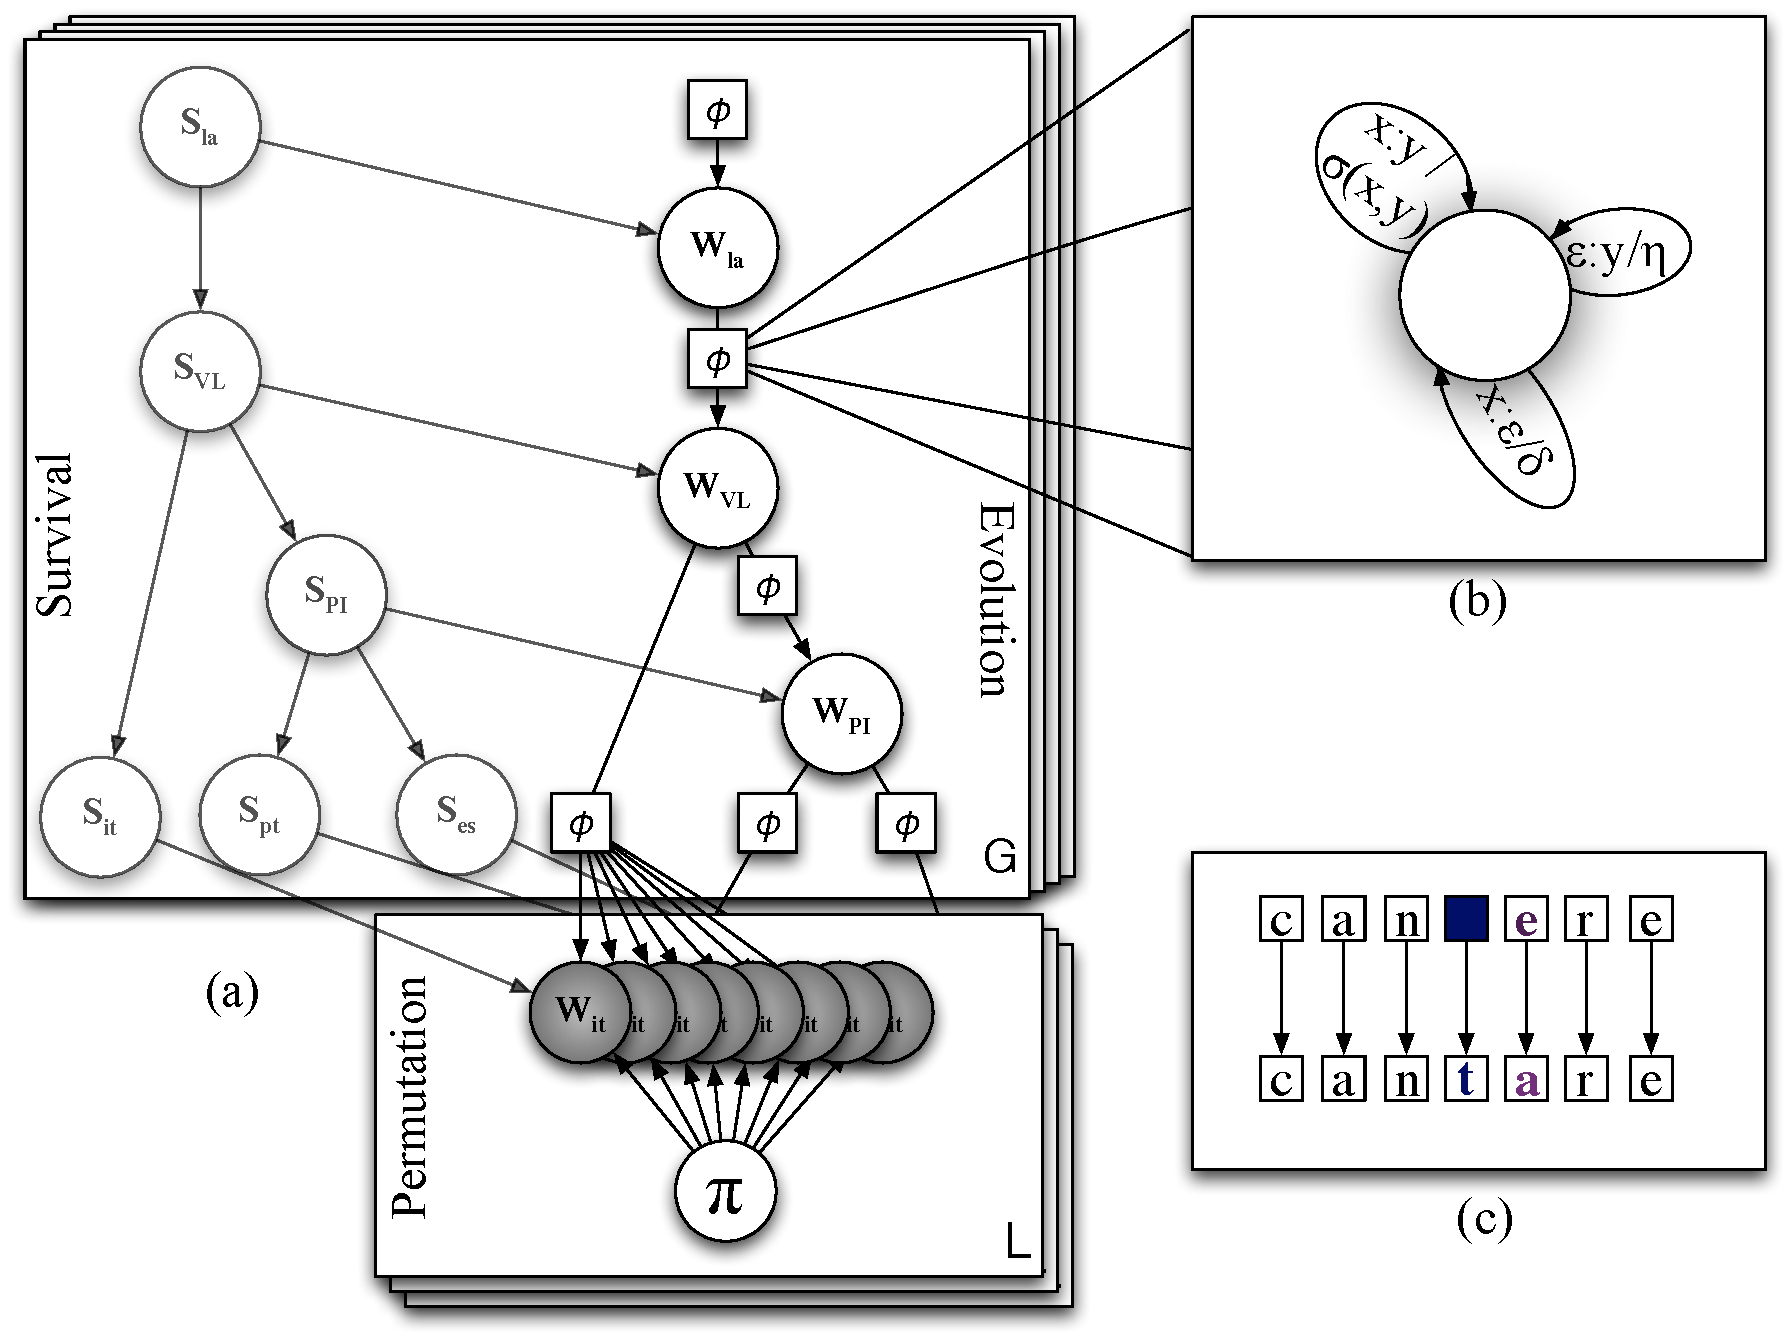
\includegraphics[scale=0.4]{gmodel}
  \caption{(a) The process by which cognate words are generated.
  Here, we show the derivation of Romance language words from their
  respective Latin ancestor. (b) A close-up of a possible alignment
  produced by a transducer. In this paper we use unigram transducers
  that are equivalent to parameterized edit distances.  (c) When
  some cognate trees may not be complete, we model the ``death''
  of words on another tree running parallel to the word-generating
  tree.}

  \label{fig:gmodel}
\end{figure*}

Our model generates words according to a transformation from their
immediate ancestor. Figure (\ref{fig:gmodel}a) graphically describes
our generative model for three Romance languages: Italian, Portuguese,
and Spanish. In each cognate group, each word $w$ is generated from
its parent using a transducer $\phi$, which is specific to that
edge in the tree, but shared between all cognate groups. For instance,
as illustrated in Figure (\ref{fig:gmodel}b), the Vulgar Latin word
\textit{cantare} is generated from its parent form \textit{canere}
by a series of edits. The probability of each individual edit is
determined by $\phi$, and the probability of the descendent Vulgar
Latin word conditioned on the Latin word is the sum over all possible
alignments that generate it.

At the leaves of the trees are the observed words. (We take interior
nodes to be unobserved.) Here, we make the (false, but simplifying)
assumption that in any language there is at most one word per
language per cognate group.  Because which words belong to which
cognate group is unknown, we specify an unknown parameter $\pi_\ell$
for each language that specifies a permutation of the words which
specifies the mapping. In this paper, our task is primarily to learn
the permutations $\pi_\ell$.

A further complication is that words in a cognate group may die off
or otherwise be unattested in a surface language. To capture this
constraint, for each cognate group we create a parallel ``death
tree'' with variables $\delta_\ell$ specifying whether or not the
word died before reaching that language. Death at any node in the
tree requires that all of that node's descendants also be dead.
This parallel tree models the intuition that a word is more likely
to be found in two sibling languages (e.g. Spanish and Portuguese)
than in two cousin languages (e.g. Portuguese and Italian) and not
an intervening sibling (Spanish).  The death tree is shown in Figure
(\ref{fig:gmodel}c).

Finally, because we do not know how many cognate groups there may
be ahead of time, we place a geometric prior on the number of
unobserved groups. (XXX)

\subsection{Inference}

We are given a set of languages and a list of words
in each language, and our objective is to determine which words are
cognate with each other words. In the Romance dataset, we have the
additional constraint that each cognate group supports exactly one
word from each language. In effect, in the Romance dataset the 
inference task is reduced to finding a permutation of the respective
word lists to maximize the log probability of the observed words:
\begin{equation}
  \begin{split}
    \vec{\pi} = \arg\!\max_{\vec \pi} \sum_{g} \log p(\vec w_{(\ell,\pi_\ell(i))}|\vec \phi,\vec \pi)
   \end{split}
 \end{equation}
Maximizing this equation directly is intractable, and so instead
we use a coordinate ascent algorithm to iteratively maximize one
permutation while holding the others fixed:
\begin{equation}
  \begin{split}
    \pi_\ell = \arg\!\max_{\pi_\ell} \sum_{g} \log p(\vec w_{(\ell,\pi_\ell(i))}|\vec \phi,\vec \pi_{-\ell},\pi_\ell)
  \end{split}
\end{equation}
Each iteration is then actually an instance of bipartite graph
matching, with the words in one language one set of nodes, and the
current cognate groups in the other languages the other set of
nodes, and the edge affinities between these nodes are the conditional
probability of each word belonging to each cognate group. To compute
the affinities for each cognate group, inference in each tree
computes the marginal distribution of the words from the ``held
out'' language, and likelihoods are computed for each word.  Given
these weights, we use the Kuhn-Munkres algorithm (XXX cite ) algorithm
to find an approximate maximizer.

One important note is initialization. In our early experiments we
found that choosing a random starting configuration usually led to
rather poor local optima. Instead, we started with empty trees, and
added one language in per iteration until all languages were added,
and then continued iterations on the full tree.

\subsection{Message Approximation}

Unfortunately, the maximal number of states in a message in each
cognate group is exponential in the number of words assigned to
that group. Minimization can only help so much: in order for two
states to be collapsed, the distribution over transitions from those
states must be indistinguishable, or indistinguishable to within
some tolerance. In practice, for the kinds of transducers generated
in our model, minimization removes at most half the states, which
is not sufficient to counteract the exponential growth. Thus, we
need to find a way to approximate a message $\mu(x)$ by some simpler
distribution $\hat\mu(x;\theta)$, which has some simpler form with
parameter $\theta$.

In the context of transducers, previous authors have focused on a
combination of n-best lists and unigram\footnote{Here, and for the
rest of the paper, the ``grams'' of interest are characters in the
International Phonetic Alphabet.} back-off models. (XXX cite eisner)
In our setting, n-best lists seem inadequate; early experiments
showed that a 10,000-best list for a typical message only accounts
for 50\% of message log perplexity. That is, the posterior marginals in
our model are fairly flat.

An alternative approach might be to simply treat messages as
unnormalized probability distributions, and to minimize the KL
divergence between some approximating message and the true message.
However, messages are not always probability distributions and--because
the distribution over potential strings is in principle infinite--they
need not sum to a finite number. Instead, we propose to minimize
the KL divergence between the ``expected'' marginal distribution
and the approximated ``expected'' marginal distribution:
\begin{equation}
  \begin{split}
    \hat\theta &= \arg\!\min_{\theta} D_{KL}(\tau(w)\hat\mu(w;\theta)||\tau(w)\mu(w) ) \\
    &= \arg\!\min_{\theta} \sum_w \tau(w) \hat\mu(w;\theta) \log \frac{\tau(w)\hat\mu(w;\theta)}{\tau(w)\mu(w)} \\
    &= \arg\!\min_{\theta} \sum_w \tau(w) \hat\mu(w;\theta) \log \frac{\hat\mu(w;\theta)}{\mu(w)} \\
   \end{split}
 \end{equation}
where $\tau$ is a prior distribution acting as a surrogate for the posterior
distribution over $w$ without the information from $\mu$. That is, we 
seek to approximate $\mu$ not on its own, but as it functions in
an environment representing its final context. 

In the context of this paper, $\mu(w)$ is a complex automaton with
potentially many states, $\hat\mu(w)$ is a simple parametric automaton
with forms that we discuss below, and $\tau(w)$ is an arbitrary
(but hopefully fairly simple) automaton.  The actual method we use
is as follows. Given a deterministic prior transducer $\tau$, and
a deterministic automaton topology $\hat\mu^*$, we created the
composed unweighted automaton $\tau \circ \hat \mu^*$, and calculate
arc transitions weights to minimize the KL divergence between that
composed transducer and $\tau\circ\mu$.  The procedure for calculating
these statistics was described in (XXX cite the other eisner paper),
which amounts to using an expectation semiring (XXX cite yet another
eisner paper) to compute expected transitions in $\tau\circ\mu$.

From there, we need to created the transducer
$\tau^{-1}\circ\tau\circ\hat\mu$. That is, we need to divide out
the influence of $\tau(w)$. Since we know the topology and arc
weights for $\tau$ ahead of time, this is often as simple as dividing
arc weights in $\tau\circ\hat\mu$ by the corresponding arc weight
in $\tau(w)$. For example, if $\tau$ encodes a geometric distribution
over word lengths and a uniform distribution over characters (that
is, $\tau(w) \propto {p^{|w|}}$), then computing $\hat\mu$ is as
simple as dividing each arc in $\tau\circ\hat\mu$ by
$p$.\footnote{Actually, we must be sure to divide each ``final
weight'' in the transducer by $(1-|\Sigma| p)$}

There are a number of choices for $\tau$. One is a hard maximum on the
length of words. Another is to choose $\tau(w)$ to be a unigram
language model over the language in question with a geometric
probability over lengths. In our experiments, we find that $\tau(w)$
can be a \textit{uniform} distribution over characters and still
obtain reasonable results.


\section{Learning}

So far we've only addressed learning the permutations $\pi$ and
the approximations needed to perform inference tractably. We also
have two other sets of parameters: the transducers $\phi$, and the
death probabilities $\delta$. The parameters can be learned through
standard maximum likelihood estimation, which we detail in this
section.

Estimating the parameters for each $\delta_\ell$ is straightforward.
Because we enforce that a word must be dead if its parent word is
dead, we simplify need to learn the conditional probabilities
$p($death$|$parent not dead$)$. Given fixed assignments $\pi$, we
simply count, apply smoothing (we found XXX to be a good value) and
divide.

Estimating the parameters for each transducer can be performed
analogously to the message approximation algorithm presented in the
previous section without the need for the extra prior distribution
$\tau$. For each pair of parent/child languages $(a,d)$ and each
cognate group $g$, we maintain a factor marginal as a transducer.
Our goal is to compress these G factor marginals into a single
transducer that best approximates the alignments seen across all
cognate groups.

In this paper, we learn parameterized edit distances which are
essentially Levenshtein distances with a non-uniform substitution,
insertion, and deletion matrix. These edit distances define a
exponential family distribution when conditioned on an ancestral
word (or when multiplied by a prior distribution over those words).
To construct the transducers, we follow a similar approach to the
approach described for messages, but two essential differences hold.
First, we must tally expected ``alignment n-grams'' rather than
character n-grams. Second, we do not need to use the new loss
function, because the messages are normalized and we know what what
the arcs must sum to. Based on the description in (XXX cite the
edit distance paper I found), we have that, for each character $a$
in the ancestor language:
\begin{equation}
  \begin{split}
    \sum_{b \in \Sigma \cup \{\epsilon\}} w(a,b) &= 1 - \sum_{b \in \Sigma} w(\epsilon,b) \\
    w(a,b) &\propto \frac{\#(a,b)}{\#(a,\cdot)} \\
    w(\epsilon,b) &\propto \frac{\#(\epsilon,b)}{\#(\cdot,\cdot)} \\
   \end{split}
 \end{equation}
where $\#(a,b)$ indicates the expected number of times the alignment
of $a$ and $b$ are seen. These equations ensure that the three transition
types (substitution/match, deletion, and insertion) are normalized for
any ancestral character.

\section{Experiments}

\subsection{Baseline}

\subsection{Experiment 1: Romance}

XXX some text


For evaluation, we report two metrics. The first is pairwise accuracy
for each pair of languages averaged across pairs. The other
is accuracy measured in terms of the number of correctly and
completely reconstructed cognate groups. 

Table \ref{tbl:exp1} shows the results under various configurations. XXX

\begin{table}
  \begin{tabular}{|c|c|c|c|}
    Transducers & Messages & Pair Acc. & Rec. Acc.\\
    \hline
    \hline
    Levenshtein&Unigrams & & \\
    Levenshtein&Pos. Unigrams & & \\
    Levenshtein&Bigrams & & \\
    Levenshtein&K-Best & & \\
    \hline
    Learned&Unigrams & & \\
    Learned&Pos. Unigrams & & \\
    Learned&Bigrams & & \\
    Learned&K-Best & & \\
  \end{tabular}
  \caption{Accuracies for reconstructing cognate groups. Levenshtein
  refers to fixed parameter edit distance transducers with
  deletion/insertion and substitution costs set to XXX, respectively.
  Learned refers to automatically learned edit distances.}
  \label{tbl:exp1}
\end{table}

\subsection{Experiment 2: Austronesian}

\subsection{Experiment 3: Reconstructions}


\section{Previous Work}
XXX expand and cite:

1) The reconstruction engine: a computer implementation of the
comparative method\\
  A deterministic approach from 1994 designed to help linguists look
at reconstructions. Closer to Alex's stuff. \\
2) Automatic Detection of Orthographic Cues for Cognate Recognition (2006) \\
  Given a list of english/german words (translations of each other),
are they cognate? Pretty crappy paper.\\
3) Identifying Cognates by Phonetic and Semantic Similarity \\
  The most similar. Given a list of multiple words from four Native
American languages, sort out which words are cognate. Uses their
English glosses to look up WordNet distance in addition to phonetic
distances. Phonetic distances are measured either using DICE on
bigrams, Longest Common Subsequence, and then a kind of edit distance
on phone classes (that was earlier work he borrowed. ALINE) *DICE on
bigrams and LCS look like good baselines.*\\
  -- This approach was geared towards precision/recall, and in some
sense is the real task. I'll see if I can find the data. \\
4)  Combining Evidence in Cognate Identification (2004) \\
  A very similar paper to (3). Uses ALINE to do phonetic comparisons.
Doesn't compute proto-projections like we do. Direct comparison of
words. Performance in the 50-65\% Average Precision range.\\
5) Minimally Supervised Morphological Analysis by Multimodal Alignment (2000) \\
  Basically does what Eisner and his student did on pairwise entries,
so no graphical model.\\
6) Semi-Supervised Learning of Partial Cognates using Bilingual Bootstrapping
  Basically context driven. Different task, but probably worth mentioning.

\section{Conclusion}
\section*{References}
\bibliographystyle{acl}
\bibliography{refs}


\end{document}
